\section{Flujometrías y CFD}
%
Para obtener una mejor caracterización del funcionamiento de los puertos de
admisión y escape es necesario tener mayor conocimiento del coeficiente de
descarga $C_{D}$ en diferentes condiciones operativas de los mismos.
%
Esto se logró realizando una serie de flujometrías para obtener valores de
$C_{D}$ en función de la diferencia de presión que \emph{ve} el puerto y la
apertura del mismo\footnote{ICESym utiliza alzada, por lo que se traduce área de
pasaje de puerto en alzada de válvula equivalente.}, con el fin de obtener un
mapa en función de la presión y la alzada $C_{D} = f(\Delta P,l_v)$.

El simulador ICESym requiere de información sobre el coeficiente de descarga
para calcular el área efectiva de pasaje de flujo de las válvulas (o puertos en
el caso del MRCVC), introduciendo el mapa de coeficientes se tiene una mejor
aproximación al funcionamiento del sistema de intercambio de gases porque se
tiene un modelado de la eficiencia del sistema para distintos regímenes del
motor.

% El código del programa es accesible por los usuarios, esta es una característica
% entender cómo funcionan y qué parámetros requieren algunas de las condiciones
% de contorno y post-procesadores utilizados en este trabajo.

% Para realizar las simulaciones se utilizaron los \emph{solvers}
% \emph{pimpleFoam} para flujo incompresible y \emph{rhoPimpleFoam} para flujo
% compresible.
%
% Para la turbulencia se utilizó un modelo de dos ecuaciones
% \emph{$\kappa-\epsilon$}\parencite{wilcox}, este es uno de los más utilizados
% y por ser de dos ecuaciones es un modelo completo.
% es decir , provee una ecuación para $\kappa$ y otra para la escala de longitud
% turbulenta $l_m$.
%
% Este modelo requiere que se aproximen los valores iniciales de $\kappa$ y
% $\epsilon$, que a su vez requieren de la estimación de la longitud de mezcla o
% escala de la viscosidad $l_m$.

\subsection{Modelos de turbulencia}
% pag 99 (83)

El flujo a través del puerto es de carácter transitorio, turbulento.
%
%TODO: pongo algo de RAS?
Para modelar este tipo de flujo se utilizó el modelo de dos ecuaciones
\emph{$\kappa-\epsilon$}\parencite{wilcox}, que brinda una ecuación para la
\emph{energía cinética turbulenta} $\kappa$ y otra para la \emph{velocidad de
disipación de la energía cinética turbulenta} $\epsilon$.
%
El modelo está basado en el modelo estándar
$\kappa-\epsilon$~\parencite{launderSpalding}, es uno de los más populares con
\emph{performance} conocida y las ecuaciones del modelo son

\begin{equation}\label{eq:k}
  \frac{D}{Dt}(\rho \kappa) = \nabla \cdot (\rho D_{\kappa}\nabla \kappa) + P - \rho \epsilon
\end{equation}

Dónde:
$\kappa$ es la energía cinética turbulente en $m^{2}s^{-2}$
$D_{\kappa}$ es la difusividad efectiva para $\kappa$
$P$ es la velocidad de producción de energía cinética turbulenta en $m^{2}s^{-3}$
$\epsilon$ es la velocidad de disipación de energía cinética turbulenta en $m^{2}s^{-3}$


\begin{equation}\label{eq:k}
  \frac{D}{Dt}(\rho \epsilon) = \nabla \cdot (\rho D_{\epsilon}\nabla \epsilon) \frac{C_{1}\epsilon}{\kappa} \left( P+C_{3}\frac{2}{3}\kappa\nabla\cdot u \right) - C_{2}\rho\frac{\epsilon^{2}}{\kappa}
\end{equation}

Dónde: 1) $D_{\epsilon}$ es la difusividad efectiva de $\epsilon$, 2) $C_{1}$ es
un coeficiente del modelo, 3) $C_{2}$ es un coeficiente del modelo.

La ecuación para la viscosidad turbulenta $\nu_{t}$ es

\begin{equation}\label{eq:nu_t}
  \nu_{t} = C_{\mu}\frac{\kappa^{2}}{\epsilon}
\end{equation}

Dónde: 1) $C_{mu}$ es un coeficiente del modelo, 2) $\nu_{t}$ es la viscosidad
turbulente en $m^{2}s^{-1}$.

Los coeficientes por defecto del modelo son

% Clossure Coefficient
\begin{equation}
  C_{\epsilon 1}=1.44
  \quad
  C_{\epsilon 2}=1.92
  \quad
  C_{\mu}=0.09
  \quad
  \sigma_{k}=1
  \quad
  \sigma_{\epsilon}=1.3
\end{equation}

El valor inicial para $\kappa$ se puede estimar con:
\begin{equation}\label{eq:kappa_est}
  \kappa = \frac{3}{2} {\left( |u_{ref}| \cdot I \right)}^{2}
\end{equation}

Dónde: 1) $I$ es la intensidad de turbulencia en \%, 2) $u_{ref}$ es una
velocidad de referencia en $ms^{-1}$.

El valor inicial para $\epsilon$ se puede estimar con:
\begin{equation}\label{eq:epsilon_est}
  \epsilon = \frac{{C_{\mu}}^{3/4} \cdot {\kappa}^{3/2}} {l_{m}}
\end{equation}

Dónde: 1) $C_{\mu}$ es una constante del modelo que valo 0.09 por defecto, 2)
$l_{m}$ es una longitud de referencia, para flujos internos se estima con el
diámetro hidráulico de la cañería, $0.07\cdot D_{m}$.

% % Auxiliary Relations
% \begin{equation}
%   w = \epsilon/(C_{\mu}k)
%   \quad
%   \textrm{y}
%   \quad
%   l = C_{\mu}k^{3/2}/\epsilon
% \end{equation}

% Y los coeficientes utilizados en este trabajo son los siguientes:

% \begin{align*}
%     %
%   C_{\mu} &= 0.09 \\
%     %
%   I &= 0.05 \\
%     %
%   l_{m} &= 0.07 \cdot D_{m} \\
%   %
%   \kappa &= 1.5 \cdot {\left( u_{ref} \cdot I \right)}^{2}\\
%     %
%   \epsilon &= \frac{{C_{\mu}}^{3/4} \cdot {\kappa}^{3/2}} {l_{m}}
%     %
% \end{align*}

% Dónde:
% %
% \begin{itemize}

%     \item $C_{\mu}$, es un coeficiente propio del modelo.
%         %
%     \item I, es la intensidad de turbulencia estimada, se utilizó 0.05.
%         %
%     \item $l_m$, es la longitud de mezcla o escala de viscosidad,
%      para flujos internos se suele usar el diámetro hidráulico de la cañería.
%         %
%     \item $u_{ref}$, es la velocidad de referencia del flujo en m/s.
%         %
%     \item $\kappa$, es la energía cinética turbulenta.
%         %
%     \item $\epsilon$, es la disipación de energía cinética turbulenta.
%         %
% \end{itemize}

% %
% % https://www.openfoam.com/documentation/guides/latest/doc/guide-turbulence-ras-k-epsilon.html

Las ecuaciones anteriores de  $\kappa$ y $\epsilon$ son estimaciones para dar un
valor inicial al problema.
%
La longitud de mezcla $l_m$ determina el tamaño que pueden tener los
\emph{eddys} turbulentos, su valor inicial se aproximó como la altura de cámara
$l_m = h_c$.

\subsection{Condiciones Iniciales}\label{cap2:cond_iniciales}
%
Las condiciones iniciales se determinan para cada punto de interés a partir de
los datos obtenidos del simulador ICESym.
%
Se tienen dos casos distintivos al momento de modelar el flujo a través de los
puertos, flujo compresible e incompresible.
%
Para este último se considera que los efectos de la compresibilidad del gas se
pueden despreciar cuando el número de Mach es menor a $0.3-0.4$.
%
Además, se deben separar los casos a modelar entre aquellos en los que hay
solape de cámaras y los que no (ver figura~\ref{fig:solape}), en estos casos se
define también un valor medio para inicializar el interior del dominio que
representa el gas dentro de la cámara de combustión.

\begin{figure}[t!]
  \centering
    \begin{subfigure}[t]{0.4\textwidth}
        \centering
        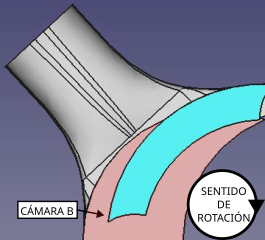
\includegraphics[width=\textwidth]{flujometrias/sin_solape.png}
        \caption{Sin solape}
    \end{subfigure}%
    \begin{subfigure}[t]{0.4\textwidth}
        \centering
        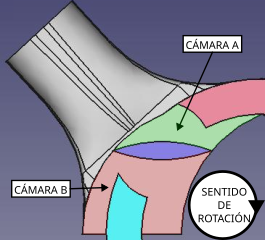
\includegraphics[width=\textwidth]{flujometrias/con_solape.png}
        \caption{Con solape}
    \end{subfigure}
  \caption{Solape de cámaras}\label{fig:solape}
\end{figure}

Independientemente del tipo de flujo que se esté simulando, de ICESym se toman
los valores de presión, temperatura, densidad y velocidad para calcular los
valores iniciales.
%
% En la tabla~\ref{tab:condiciones_iniciales} se muestran los datos necesarios
% para las flujometrías, separados en flujo incompresibles (pimpleFoam) y
% compresibles (rhoPimpleFoam).

% \begin{table}
% \centering
    % \begin{tabular}{rccc} \toprule
    %   Variable      & Descripción   & Incompresible & Compresible \\ \midrule
    %   $\epsilon$    &               &               & \\
    %   $\kappa$      &               &               & \\
    %   $\gamma$      &               &               & \\
    %   $\mu$         &               &               & \\
    %   $\nu$         &               &               & \\
    %   $M_{w}$       &               &               & \\
    %   $P_{r}$       &               &               & \\
    %   $\rho$        &               &               & \\
    %   $P_{puerto}$  &               &               & \\
    %   $P_{cámara}$  &               &               & \\
    %   $V_{puerto}$  &               &               & \\
    %   $T_{puerto}$  &               &               & \\
    %   $T_{cámara}$  &               &               & \\ \bottomrule
    % \end{tabular}
    % \caption{Condiciones Iniciales}\label{tab:condiciones_iniciales}
% \end{table}

% No se considera la transferencia de calor en las paredes.

Debido a la cantidad de flujometrías a realizar, se utilizó un script para leer
los datos de salida de ICESym y calcular los valores requeridos en función del
tipo de flujo a simular.

Este script toma el estado del gas del simulador tanto en la cámara de
combustión como del puerto que se esté analizando, para la posición de alzada y
RPM requeridas.
%
Con estos valores se calculan las propiedades termodinámcicas del gas con las
siguientes relaciones para cada cámara analizada, los valores leídos son los
indicados en la tabla~\ref{tab:estado_gas_icesym}.

\begin{table}
  \centering
  \begin{tabular}{ll}\toprule
    Parámetro & Descripción \\ \midrule
    $\rho_{c,i}$ & Es la densidad del gas en la cámara de combustión $i$\\
    $P_{c,i}$ & Es la presión del gas en la cámara de combustión $i$ \\
    $T_{c,i}$ & Es la temepratura del gas en la cámara de combustión $i$ \\
    $\rho_{p,i}$ & Es la densidad del puerto $i$ \\
    $v_{p,i}$ & Es la velocidad del gas en el puerto $i$ \\
    $P_{p,i}$ & Es la presión del gas en el puerto $i$ \\ \bottomrule
    \end{tabular}
    \caption{Estado del gas leído de ICESym}\label{tab:estado_gas_icesym}
\end{table}

A partir de esta información también se calculan los valores medios, en caso de
haber solape de cámaras para el caso analizado, se utiliza el valor medio para
calcular los valores iniciales del caso.

Con estos valores iniciales se pueden calcular o estimar las propiedades
termodinámicas de la mezcla de gases frescos o quemados, dependiendo si se está
evaluando un puerto de admisión o escape, ver tabla~\ref{tab:ci_calculados}.
%

\begin{table}
  \centering
  \begin{tabular}{ll}\toprule
    Parámetro & Descripción \\ \midrule
    $M_{M}$ & Masa molar, ec.\ref{eq:mw} \\
    $C_{p}$ & Calor específico a presión constante \\
    $\gamma$ & Relación $C_{p}/C_{v}$ del gas \\
    $\mu$ & Viscosidad dinámica, ec.\ref{eq:mu} \\
    $\nu$ & Viscosidad cinemática \\
    $P_{R}$ & Número de Prandtl, ec\ref{eq:pr}\\
    $k_{est}$ & Energía cinética turbulenta, ec.\ref{eq:kappa_est} \\ \bottomrule
    $\epsilon_{est}$ & Disipación de la energía cinética turbulenta, ec.\ref{eq:epsilon_est}\\
    \end{tabular}
    \caption{Parámetros calculados para CI}\label{tab:ci_calculados}
\end{table}

Para simplificar el análisis no se tuvo en cuenta la fracción de gases
residuales, el gas ``flujado'' es siempre aire limpio o el gas quemado de una
mezcla estequeométrica de aire-combustible, siendo isooctano $C_{8}H_{18}$ el
combustible seleccionado.

Se utilizaron rutinas computacionales para modelar las propiedades
termodinámicas de las mezclas aire-combustible, descritas brevemente en
secciones anteriores, ver sección~\ref{subsec:prop_mezcla}.

\subsection{Malla}

La malla se construyó a partir del modelo de CAD generado con los resultados
obtenidos de las simulaciones del motor.

La implementación de las diferentes herramientas requeridas para generar una malla apta para realizar las flujometrías se describe en el apartado~\ref{sec:cap3_of_malla}

La malla utilizada y las características de la construcción de la misma se
describen en la sección TODO,

el grado de refinamiento de la misma se determinó
luego de realizar una serie de flujometrías con tamaños decrecientes de celda y
viendo la variabilidad de los resultados.
%
El objetivo de las flujometrías es obtener el flujo másico $\dot{m}$ del puerto
para un estado del gas dado, se redujo el tamaño inicial de celda hasta que el
valor de $\dot{m}$ no se modificó en más de un 5\% del valor anterior, con un
nivel de refinamiento mayor.
%
En algunos casos se utilizaron mallas más gruesas para obtener un valor inicial
de una malla de mayor refinamiento.
%
Por ejemplo, con una malla inicial de cubos de 15mm de lado se obtiene una
solución que se usa como valor inicial para una malla de 10mm y finalmente se
realiza la simulación con la malla de 5mm para obtener el valor final del flujo
másico.

\subsection{Coeficiente de descarga $C_{D}$}\label{sec:cap2_cd}

El flujo másico que fluja el puerto se calcula a partir de las ecuaciones de
flujo compresible a través de una restricción, habiendo dos casos distintivos:
flujo bloqueado y no bloqueado.

El flujo está bloqueado si la velocidad en la garganta de la restricción alcanza
la velocidad sónica, dada esta condición el flujo másico alcanza un límite y
reducir la presión aguas abajo de la restricción no produce un aumento del caudal.
%
La condición de flujo bloqueado se puede expresar en términos de la relación de
presiones aguas arriba $p_{0}$ y aguas abajo de la restricción $p_{T}$.
%
Si se cumple la inecuación~\ref{eq:condicion_bloqueo}, el flujo está bloqueado.

El caudal másico para la condición de no bloqueado se calcula con la
ecuación~\ref{eq:m_no_bloqueo} y la ecuación~\ref{eq:m_bloqueo} en caso de que
el flujo esté bloqueado.
%
Los parámetros involucrados en estas ecuaciones se describen en la
tabla~\ref{tab:parametros_cd}.

\begin{equation}\label{eq:condicion_bloqueo}
  \frac{p_{T}}{p_{0}} \le {\left(\frac{2}{\gamma+1}\right)}^{\frac{\gamma}{\gamma - 1}}
\end{equation}

\begin{equation}
    \label{eq:m_no_bloqueo}
    \dot{m} = \frac{C_D A_R p_0}{\sqrt{R T_0}}
            {\left(\frac{p_T}{p_0} \right)}^{1/\gamma}
            {\left( \frac{2\gamma}{\gamma-1} \left[1- {\left(\frac{p_T}{p_0}\right)}^{{\gamma-1}/\gamma} \right] \right)}^{1/2}
\end{equation}

\begin{equation}\label{eq:m_bloqueo}
  \dot{m}=  \frac {C_D A_R p_0} {{(R T_0)}^{1/2}}
            \gamma^{1/2}
            {\left( \frac{2\gamma}{\gamma+1} \right)}^{(\gamma+1)/(2(\gamma-1))}
\end{equation}


\begin{table}
  \centering
  \begin{tabular}{ll}\toprule
    Parámetro & Descripción \\ \midrule
    $p_0$ & es la presión de estancamiento antes de la restricción \\
    $T_0$ & es la temperatura de estancamiento antes de la restricción \\
    $p_T$ & es la presión estática justo después de la restricción \\
    $A_R$ & es el área de referencia \\
    $\dot{m}$ & es el caudal másico \\
    $\gamma$ & es el cociente de capacidades térmicas del gas \\ \bottomrule
  \end{tabular}
  \caption{Parámetros de
ecuaciones~\ref{eq:condicion_bloqueo},~\ref{eq:m_bloqueo},
y~\ref{eq:m_no_bloqueo}}\label{tab:parametros_cd}
\end{table}


Un parámetro importante en las ecuaciones anteriores es el área de referencia
$A_{R}$ porque define el área utilizada para calcular el caudal másico que
circula por el puerto, en un motor con válvulas se suele tomar el área de
cortina como valor de referencia que se define como el producto de la
circunferencia de la válvula ($\pi D_{v} \cdot h_{v}$) con la alzada, ver
figura~\ref{fig:area_referencia}(a).
%
El área de referencia utilizada en ICESym es el área frontal del puerto expuesta
a la cámara que se esté analizando, calculada como $A_{R} = h_{p} \cdot l_{v}$, ver
figura~\ref{fig:area_referencia}(b).

% Debido a que el MRCVC no tiene válvulas, en trabajos anteriores se confeccionó
% un script para calcular la distancia $l_{v}$ en función del ángulo del ciclo.
%
% En la figura~\ref{fig:area_referencia} se ilustran las áreas de referencia para
% una posición del rotor en la que hay solape de cámaras con $\theta = 55^{\circ}$.

\begin{figure}
    \centering
    \begin{subfigure}{0.5\textwidth}
      \centering
      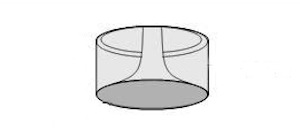
\includegraphics{valve_curtain.jpg}
      \caption{Área de cortina}
    \end{subfigure}%
    \begin{subfigure}{0.5\textwidth}
      \centering
      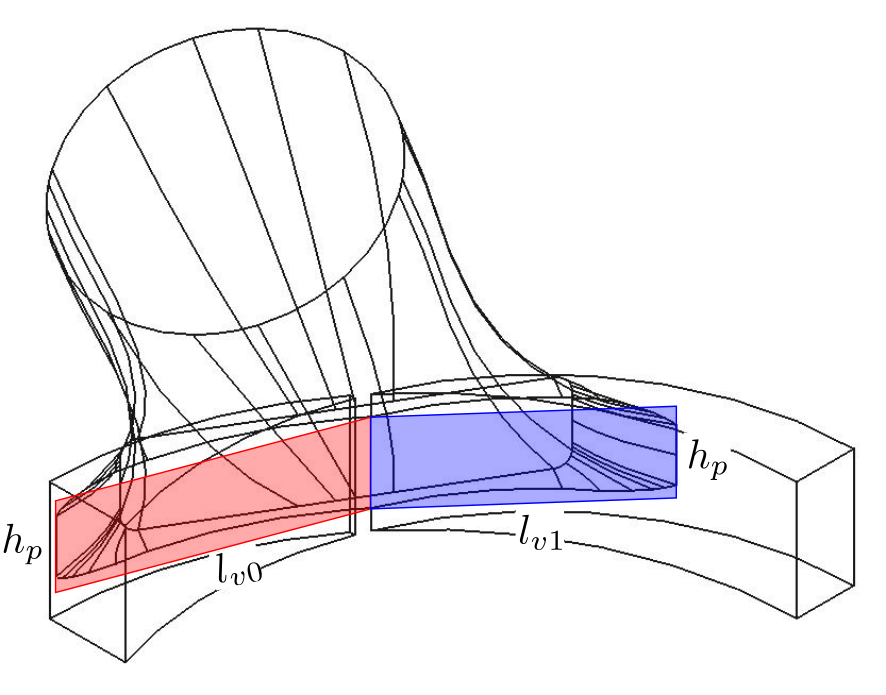
\includegraphics{area_referencia.png}
      \caption{Área de referencia MRCVC}
    \end{subfigure}
    \caption{Área de referencia}\label{fig:area_referencia}
\end{figure}

Los valores de densidad, velocidad, presión y temperatura se obtienen de los
datos de salida de ICESym para un puerto, ángulo y velocidad dada.
%
Para la temperatura se utiliza la temperatura de cámara, $T_0 = T_C$, la
presión antes y después del puerto se selecciona de acuerdo al sentido de
flujo, en caso de ser flujo hacia la cámara de combustión, la presión en el
puerto se utiliza como inicial $P_0$ y la presión en la cámara es la
aproximación a la presión en la restricción $P_T$.

El valor de $\gamma$ se obtiene de las propiedades de la mezcla con las rutinas
computacionales descritas en el apartado~\ref{subsec:prop_mezcla}.

De las flujometrías se obtiene el caudal másico que fluja el puerto, con este
dato y las ecuaciones anteriores se puede determinar el valor de $C_{D}$.

% \subsection{otro}


% Para inicializar el campo de presión y densidades, se usa la media entre las
% cámaras que se estén simulando y se establece un campo uniforme.

% La velocidad se inicializa con un campo nulo de velocidades, que en la
% configuración de OpenFOAM se designa como \emph{internalField uniform (0 0 0)}.

% En resumen, los valores iniciales de los campos de presión, temperatura y velocidad
% son los indicados en la tabla~\ref{tab:cc}.

% % \begin{table}
% % \centering
% %     \begin{tabular}{cccc} \toprule
% %         Var & Campo         & Parche                      & Pared \\
% %         T   & uniforme T0   & inletOutlet                 & uniforme T9\\ \midrule
% %         P   & uniform Pavg  & uniformTotalPressure        & Pi \\
% %         U   & uniform (0 0 0) & pressureInletOutletVelocity & valor fijo (0 0 0)\\
% %         rho & uniform rhoAvg \\ \bottomrule
% %     \end{tabular}
% %     \caption{Condiciones de Borde}\label{tab:cc}
% % \end{table}

% En todos los casos se tomará como velocidad de referencia a la media entre la
% velocidad en la punta del tubo de las cámaras solapadas.
% %
% Del mismo modo, la temperatura será la temperatura de cámara media.

% Si hay o no solape de cámaras va a depender tanto de la geometría del puerto
% como de la posición del ciclo en la que se encuentre, para determinar las
% condiciones iniciales se debe tener en cuenta el solape.
% %
% En la figura~\ref{fig:geom} se muestra un corte del puerto con un plano cuya
% normal está en $\vec{z}$, se denominará a la cámara que esté a la izquierda
% como cámara 0 y a la que esté a la derecha cámara 1.
% %
% Al haber solape de cámaras, para definir la presión del puerto y estimar las
% condiciones iniciales de los parámetros viscosos que requiere el modelo
% $k-\epsilon$ se utilizan valores medios de presión, velocidad y temperatura de
% ambas cámaras.
% %
% Además, las condiciones iniciales que se aplican al parche denominado
% \emph{puerto} es igual a la media aritmética de la velocidad de las velocidades
% de los puertos de ambas cámaras, Lo mismo sucede con la presión, densidad y
% temperatura.

% A partir de estos datos se calculan varias propiedades termodinámicas del gas,
% incluyendo la constante del gas, masa molar, viscosidad cinemática y demás.
% %
% Para calcular estas propiedades se asume que el gas no contiene gases
% residuales.

% Finalmente el caudal másico yse obtiene con OpenFOAM, en donde se simula el
% tiempo suficiente para que los caudales másicos por entradas o salidas se
% estabilice, como se ve en la figura~\ref{fig:caudalMasico}.

% \begin{figure}
%     \centering
%     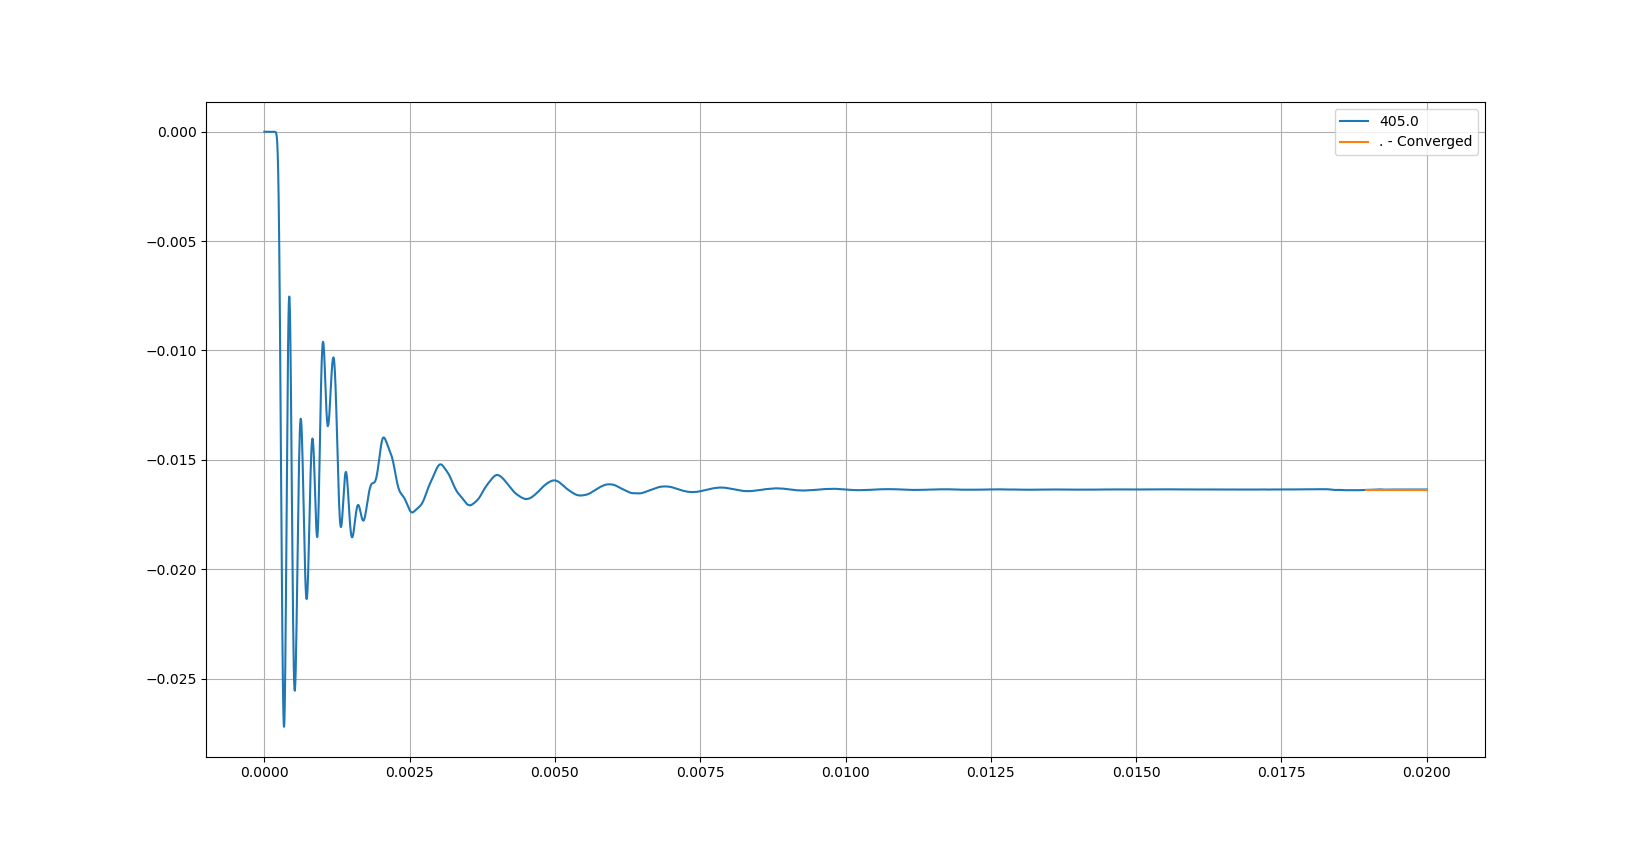
\includegraphics[width=0.6\textwidth]{surfaceFieldValue_405.0.png}
%     \caption{Flujometrías para el puerto de Admisión}\label{fig:caudalMasico}
% \end{figure}

% En todos los casos se tomará como velocidad de referencia a la media entre la
% velocidad en la punta del tubo de las cámaras que se estén solapando.
% %
% Del mismo modo, la temperatura será la temperatura de cámara media.

% Si hay o no solape de cámaras va a depender tanto de la geometría del puerto
% como de la posición del ciclo en la que se encuentre, para determinar las
% condiciones iniciales se debe tener en cuenta el solape.
% %
% En la figura~\ref{fig:geom} se muestra un corte del puerto con un plano cuya
% normal está en $\vec{z}$, se denominará a la cámara que esté a la izquierda
% como cámara 0 y a la que esté a la derecha cámara 1
% %
% Al haber solape de cámaras, para definir la presión del puerto y estimar las
% condiciones iniciales de los parámetros viscosos que requiere el modelo
% $k-\epsilon$ se utilizan valores medios de presión, velocidad y temperatura de
% ambas cámaras.
% %
% Además, las condiciones iniciales de que se aplican al parche denominado
% \emph{puerto} es igual a la media aritmética de la velocidad de las velocidades
% de los puertos de ambas cámaras, Lo mismo sucede con la presión, densidad y
% temperatura.
